\documentclass{zjureport}
\special{dvipdfmx:config z 0} % 取消PDF压缩,加快速度,最终版本生成的时候最好把这句话注释掉

% =============================================
% Part 0 Edit the info
% =============================================

\major{信息工程}
\name{黄鹤翔}
\partner{方书颖}
\title{电子电路设计实验报告}
\stuid{3230106231}
\college{信息与电子工程学院}
\date{2025-3-25}
\lab{东四216}
\course{电子电路设计实验}
\instructor{施红军/邓倩倩}
\grades{}
\expname{电流电压转换电路}
\exptype{设计型}

\usepackage{subfigure}

\begin{document}
% =============================================
% Part 1 Header
% =============================================
\makecover

% \makecontent

\makeheader
% =============================================
% Part 2 Main document
% =============================================

% \begin{figure}[H] %H为当前位置,!htb为忽略美学标准,htbp为浮动图形
%     \centering %图片居中
%     \includegraphics[width=0.8\textwidth]{fig1-SR830structure.jpg}
%     \caption{锁相放大器SR830结构图} %最终文档中希望显示的图片标题
% \end{figure}


\section{实验目的}
\begin{itemize}
  \item 熟悉电流信号转换成电压信号的原理。
  \item 掌握标准电流信号转换成电压信号的设计方法。
\end{itemize}

\section{实验任务与设计要求}
熟悉电流-电压转换电路的工作原理,并设计出一个电路,将标准电流信号 4mA~20mA 转换为标准电压信号0V~10V,误差控制在5\%以内。
\section{实验方案设计与实验参数计算}
在自动控制技术中,传感器输出的标准电流信号通常为4mA~20mA,为了便于进一步处 理,需要将其转换为0V~10V的电压信号。这可以通过工作在线性区的运算放大器来实现。
\begin{figure}[h]
  \begin{center}
  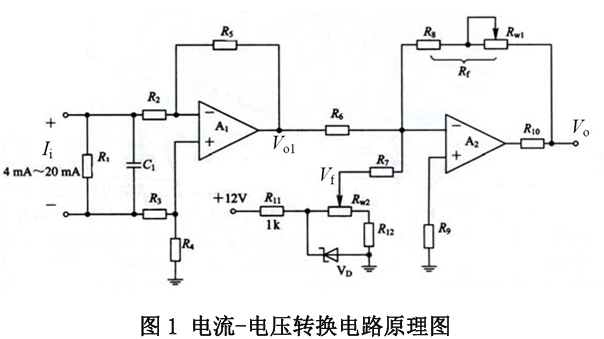
\includegraphics[width=0.8\textwidth]{原理图.png}
  \end{center}
  \caption{电流-电压转换电路原理图}
\end{figure}

\begin{itemize}
  \item 第一级放大电路:电阻R1 跨接在电流源两端,运放$A_1$采用差分输入,将4mA~20mA 的电流转换为电压。此级放大电路的放大倍数为1,输出电压$V_{o1} = -I_i*R_1$,实现了电流到电压的初步转换。
  \item 第二级放大电路:实现从$V_{o1}$到0V~10V的电平变换。根 据 对 第 二 级 电 路 的 分 析 有 :$\frac{V_{o1}}{R_6}+\frac{V_f}{R_7}=\frac{V_o}{R_f}$, 由此可推出:$V_o=\frac{R_fR_1I_i}{R_6}-\frac{R_fV_f}{R_7}$ 
  通过合理选取$R_6,R_7$的阻值,并调整$V_f$和$R_f$的值,可以确保当输入电流$I_i$从4mA变 化到20mA时,输出电压$V_o$从0V变化到10V。
  
\end{itemize}

\section{实验方案设计}

\subsection{总体参数}
\begin{math}
  V_o = \frac{R_fR_1I_i}{R_6}-\frac{R_fV_f}{R_7}
\end{math}
为了让输入电流$I_i$从$4mA$到$20mA$变化,$V_f$从$0$到$10V$变化,取
\begin{math}
  \frac{R_fR_1}{R_6} = 625\Omega\\
  \frac{R_fV_f}{R_7} = 1.25
\end{math}

\subsection{$R_1\text{、}R_2\text{、}R_3\text{、}R_4\text{、}R_5$选择}

差动放大器的四个匹配电阻$R_2\text{、}R_3\text{、}R_4\text{、}R_5$可以预先取定位中等阻值$10k\Omega$。\par

电阻$R_1$采用变送器标准负载,取$R_1 = 250\Omega$。

\subsection{$R_f$选择}
\begin{math}
  \frac{R_fR_1}{R_6} = 625\Omega
\end{math}
可取$R_6 = 10k\Omega$。

$R_f$可由$20k\Omega$固定电阻串联一个$10k\Omega$电位器$R_{w1}$得到。

\subsection{$R_6\text{、}R_7\text{、}V_f$选择}
取$R_6 = R_7 = 10k\Omega$,为了使得$I_i = 4mA\text{、}V_{o1} = -1V$时,$V_o = 0V$,取$V_f = 1V$。

\subsection{$R_{11}\text{、}R_{12}\text{、}R_{w2}$选择}
为了使得调整后的$V_f$不受电源电压变化影响,$V_f$由稳压电路分压产生\par

由于击穿电压在 4~7V 的稳压二极管温度系数最小\text{、}近似为零,这里选用 5.1V 稳压管来实现稳压电路。\par

分压后要产生 1V 左右的可调电压,分压电路可由上固定电阻串联下电位器构成。取流过分压电路电流为 5mA,则分压电路总电阻约为$1k\Omega$。若取上固定电阻 $R_{12}=510\Omega$,下电位器 $R_{w2} = 500\Omega$,则分压$V_f$将可在 0~2.5V 之间可调。

\subsection{电源\text{、}$R_{11}$\text{、}电容\text{、}补偿电阻选择}
为避免运放输出最大电压时接近饱和,运放供电电压可取为$\pm 12V$

补偿电阻$R_9 = R_6||R_7||R_f = 4.3k\Omega$\par

设稳压管最小工作电流为 10mA,则稳压管限流电阻 
\begin{math}
  R_{11} = (13V - 5.1V)/(10mA+5mA)\approx527\Omega
\end{math}
可取为标称值 $510\Omega$\par

电容主要作用是抑制高频干扰,可取为$100pF$

\section{主要仪器设备}
Multisim14.3,Altium Designer23

\section{电路仿真}

\subsection{完整实验电路}
\begin{figure}[H]
  \begin{center}
  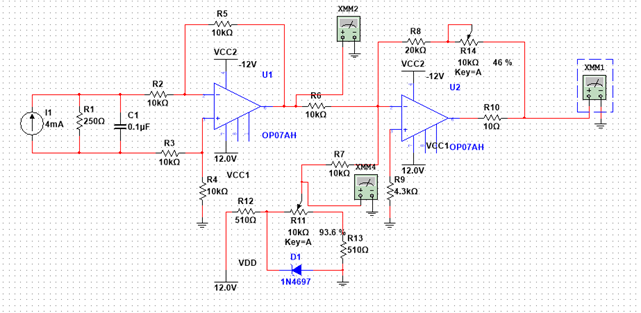
\includegraphics[width=0.8\textwidth]{multisim.png}
  \end{center}
  \caption{仿真电路}
\end{figure}

\subsection{$V_f = 1V$}
\begin{figure}[h]
  \begin{center}
  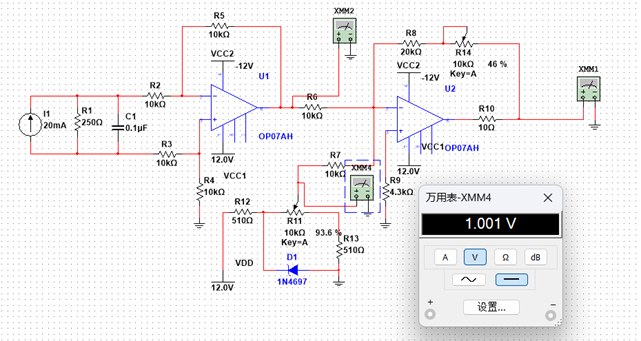
\includegraphics[width=0.8\textwidth]{仿真1.png}
  \end{center}
  \caption{$V_f = 1V$}
\end{figure}

\newpage
\subsection{输入输出测试}
\begin{figure}[h]
  \begin{minipage}{0.45\linewidth}
    \centering
    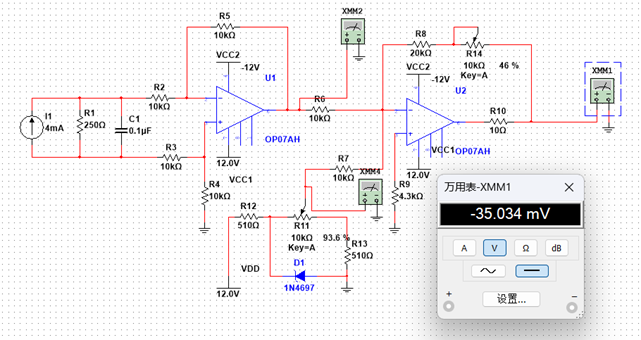
\includegraphics[width=0.8\linewidth]{仿真2.png}
    \caption{输入输出测试1}
  \end{minipage}
  \begin{minipage}{0.45\linewidth}
    \centering
    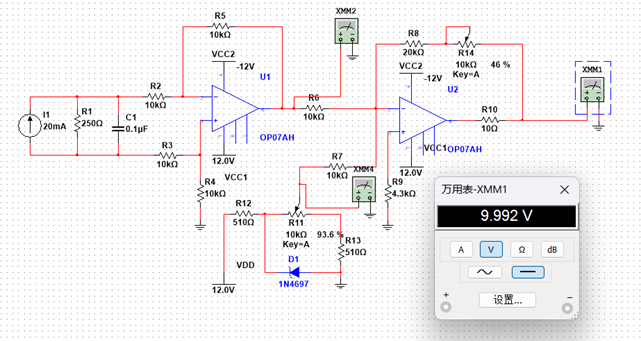
\includegraphics[width=0.8\linewidth]{仿真3.png}
    \caption{输入输出测试2}
  \end{minipage}
  \caption{输入输出测试}
\end{figure}

\section{AD设计}
\subsection{原理图设计}
原理图设计如下图所示,其中三个接插件用来输入电流、为运放供电、留出测试点
\begin{figure}[H]
  \begin{center}
  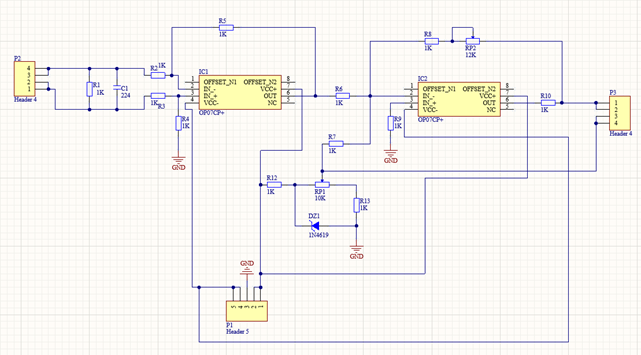
\includegraphics[width=0.8\textwidth]{ad原理图.png}
  \end{center}
  \caption{AD原理图}
\end{figure}

\subsection{PCB设计}
初版PCB设计如下图所示
\begin{figure}[H]
  \begin{center}
  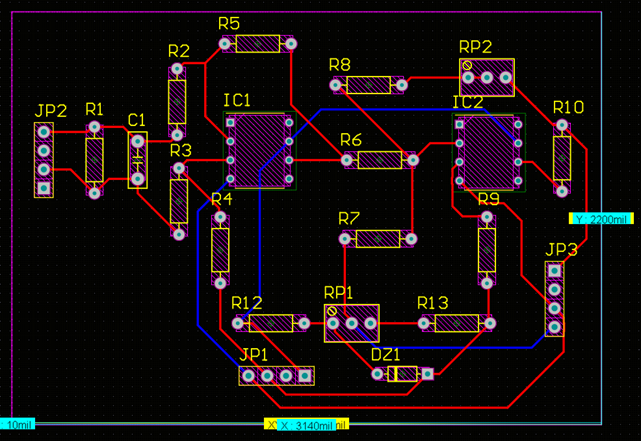
\includegraphics[width=0.8\textwidth]{pcb0.png}
  \end{center}
  \caption{初版pcb设计}
\end{figure}

改进后PCB设计如下图所示
\begin{figure}[H]
  \begin{center}
  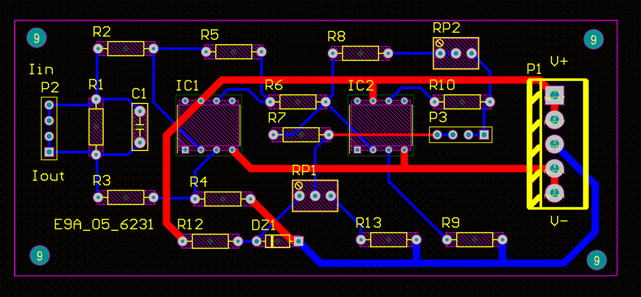
\includegraphics[width=0.8\textwidth]{pcb.png}
  \end{center}
  \caption{pcb设计改进}
\end{figure}
\end{document}